\documentclass{Dokumentmall}
\usepackage{xcolor}


\newcommand{\version}{Version 1.0}
\author{Hadi Ansari, \url{hadan326@student.liu.se}\\
  Vincent Ahlström, \url{vinah331@student.liu.se}}
\title{Språkdokumentation}
\date{2021-05-25}
\rhead{Hadi Ansari\\
Vincent Ahlström}

\begin{document}
\projectpage
\tableofcontents
\thispagestyle{empty}
\cleardoublepage
\setcounter{page}{1}
\section{Introduktion}
I den här rapporten skriven som en del av kursen TDP019 Projekt: Datorspråk, kommer programmeringsspråket Gameparser dokumenteras. Projektet Datorspråk är det tredje projektet i programmet innovativ programmering och det handlar om att utveckla ett eget datorspråk. Projektet utvecklades av en grupp av två IP-studenter under andra perioden av vårterminen 2021.

Språket är designat för (men ej begränsat till) att skapa textbaserade spel. Det har sin grund i Ruby där det via rdparse.rb översätter skriven kod till Ruby för körning. Syntaxen är inspirerad av både Ruby och Python vilket gör språket användarvänligt. Gameparser ämnar att erbjuda användaren alla verktyg som krävs för att designa en interaktiv och levande spelvärld i ett textbaserat format.

\subsection{Syfte}
Projektet ämnade ge deltagarna djupare förståelse för hur programmeringsspråk exekveras samt hur olika designval kan påverka dessa.

\subsection{Målgrupp}
Gameparser är skapat för individer som vill skapa textbaserade spel och har programmerat lite innan. För den något mer erfarne programmeraren möjliggör Gameparser skapandet av egna funktioner och klasser.

\newpage
\section{Användarhandledning}
Här beskrivs hur språket kan installeras och användas samt information om vilka konstruktioner och  datatyper språket har stöd för.

\subsection{Installation}
För att kunna komma igång med systemet två verktyg behöver installeras:
\begin{enumerate}  
\item Installera Ruby (version 2.7 rekommenderas)
\item Installera \textbf{fim} med \textbf{``sudo apt-get install fim''}.
\end{enumerate}

Gameparser kan köras interaktivt genom att skriva \textbf{``ruby gameparser.rb''} i kommandotolken (se figur 1). Kod (spel) skrivs med fördel i separata dokument som sedan körs via \textbf{``ruby gameparser.rb filväg''}. Figur 2 visar hur ett spel i ett separat dokument kan köras med Gameparser.
\begin{figure}[h!]
  \centering
  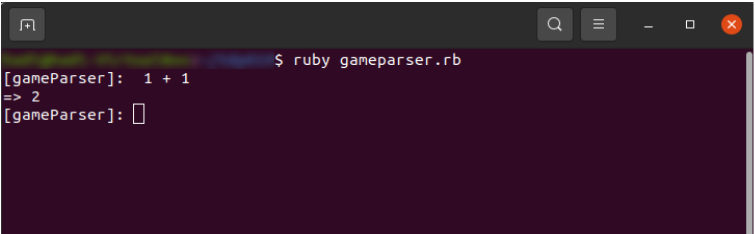
\includegraphics[scale = 0.65]{Images/Figur1.png}
  \label{}
  \caption{Att köra Gameparser i interaktivt-läge}
\end{figure}

\begin{figure}[h!]
  \centering
  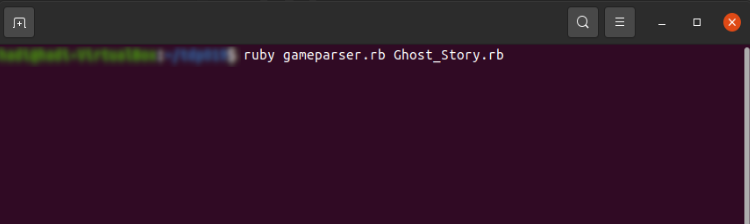
\includegraphics[scale = 0.65]{Images/Figur2.png}
  \label{}
  \caption{Att köra ett spel med Gameparser}
\end{figure}

\subsection{Konstruktioner}
Språket har stöd för villkorssatser, repetitionssatser, funktioner och rekursion, enkla klasser och verktyg för att arbeta med listor samt några fördefinierade funktioner. 
Med hjälp av en kombination av dessa verktyg har programmeraren möjlighet att designa ett unikt spel.

\subsection{Datatyper}
Gameparser har stöd för följande datatyper:
\begin{itemize}  
\item \textbf{Integer:} som kan vara ett heltal (både positiva och negativa)
\item \textbf{Sträng:} som kan vara en sträng av vilka karaktärer som helst (inklusive svenska bokstäver o.s.v)
\item \textbf{Bool:} som kan antingen vara sann eller falsk
\item \textbf{Lista:} som är en samling av olika datatyper inom hakparenteser
\item \textbf{Range:} som är en spektrum av heltal med ett specificerat start/slut-värde.
\end{itemize}

Notera att en range kan båda inkludera och exkludera slutvärdet (se figur 3). I språket kan även en range som har ett större startvärde än slutvärdet skapas.
\begin{figure}[h!]
  \centering
  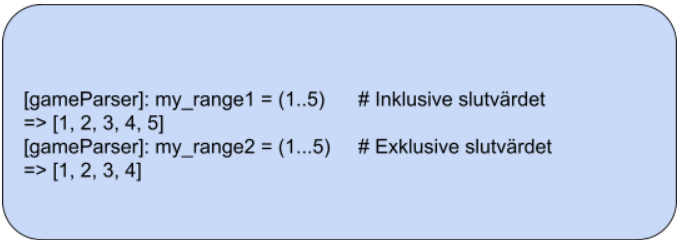
\includegraphics[scale = 0.65]{Images/Figur3.png}
  \label{}
  \caption{Exempel på hur en range kan båda inkludera och exkludera slutvärdet}
\end{figure}

I avsnittet “Variabler” kommer fler exempel på hur dessa datatyper kan användas för att kunna deklarera olika typer av variabler.

\newpage
\section{Språkstruktur}
Gameparser som språk är väldigt fritt. Ett helt spel skulle kunna skrivas på en rad om så önskas. Det finns därmed inga krav på indentering. Däremot har verktyg så som funktioner och klasser krav på hur de ska se ut. Block {} används för att köra kod medan parenteser markerar parametrar och prioriteringsordningar. 

\subsection{Kommentar}
Gameparser tillåter kommentarer i koden för att programmeraren ska kunna förtydliga sin kod. Kommentarer representeras med ett \textbf{``\#''} tecken framför kommentaren (se figur 4).

\begin{figure}[h!]
  \centering
  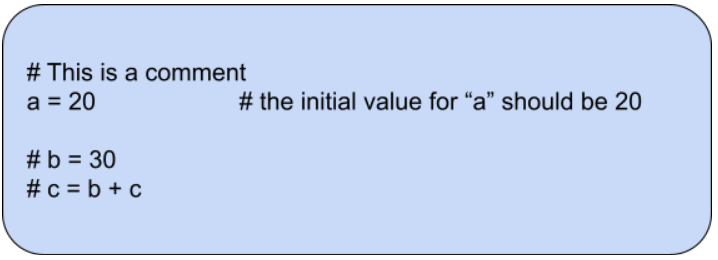
\includegraphics[scale = 0.65]{Images/Figur4.png}
  \label{}
  \caption{Exempel på hur koden kan kommenteras}
\end{figure}

\subsection{Variabel}
Deklaration av en variabel är väldig enkelt. Ett variabelnamn (identifierare) inleds med en bokstav och namnet får inte vara ett reserverad nyckelord i språket. I figur 5 visas deklaration av olika typer av variabler.

\newpage
\begin{figure}[h!]
  \centering
  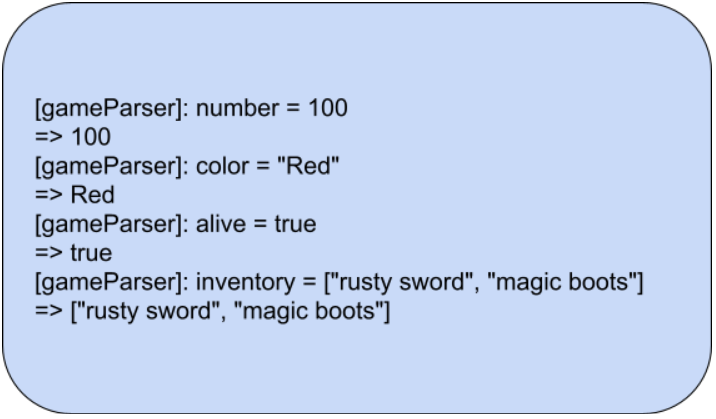
\includegraphics[scale = 0.65]{Images/Figur5.png}
  \label{}
  \caption{Exempel på deklaration av olika variabeltyper}
\end{figure}

Språket har ett dynamiskt typsystem vilket innebär att det inte finns strikta regler för att definiera variabler när det gäller typ. Det gör så att en typkontroll sker under exekvering. Därmed är det möjligt att skapa variabler av olika typer och ändra dem genom att tilldela ett annat värde av en annan typ om så önskas (se figur 6).

\begin{figure}[h!]
  \centering
  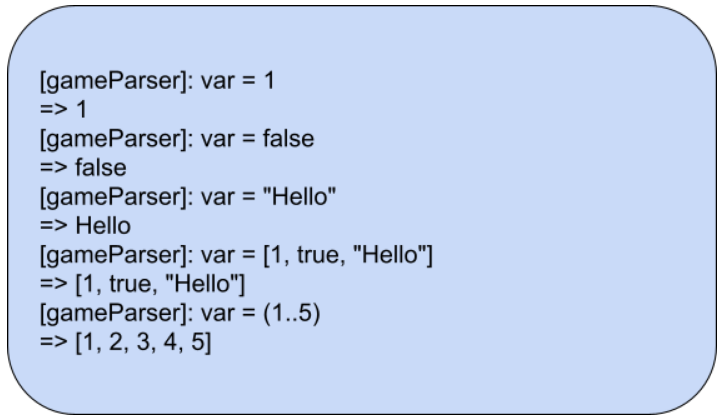
\includegraphics[scale = 0.65]{Images/Figur6.png}
  \label{}
  \caption{Dynamisk typsystem i Gameparser}
\end{figure}

\newpage
Det är även möjligt att göra en variabel-tilldelning med hjälp av variabler som redan har definierats (se figur 7).
\begin{figure}[h!]
  \centering
  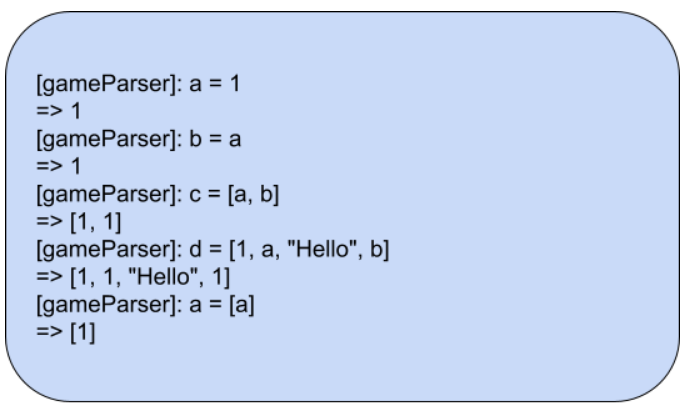
\includegraphics[scale = 0.65]{Images/Figur7.png}
  \label{}
  \caption{Deklaration av nya variabler med existerande variabler}
\end{figure}


\newpage
Språket har stöd för en form av scope-hantering så att variabler i en funktion till exempel kan nås inom den ramen som är rimlig för dem. Samma regler gäller för andra konstruktioner så som \textbf{``event''} och  \textbf{``prop''}. De har sina egna lokala variabler som inte kan nås utanför den rimliga ramen. Scope-hantering förklaras under rubriken “Scope” längre ned i dokumentationen.

I språket kan programmeraren skapa variabler i ett globalt scope som kan kallas var som helst i koden. Globala variabler definieras med hjälp av ett ``\$'' tecken som förekommer framför variabel-namnet (se figur 8).

\begin{figure}[h!]
  \centering
  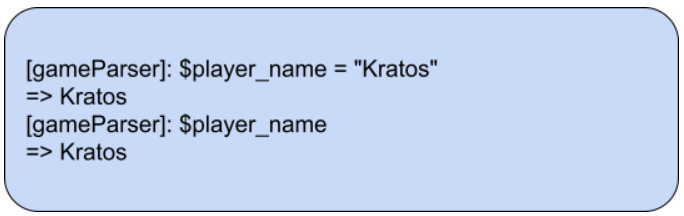
\includegraphics[scale = 0.65]{Images/Figur8.png}
  \label{}
  \caption{Deklaration av globala variabler}
\end{figure}

Alla regler som gäller vanliga variabler gäller även globala variabler. Den enda skillnaden är att globala variabler är tillgängliga överallt i koden och inte är beroende på scope (se figur 9).

\begin{figure}[h!]
  \centering
  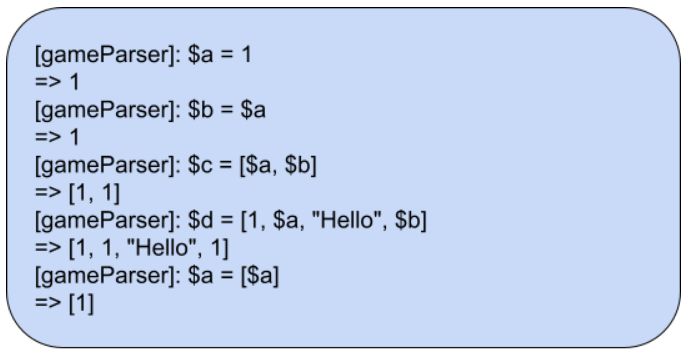
\includegraphics[scale = 0.65]{Images/Figur9.png}
  \label{}
  \caption{Deklaration av nya globala variabler med existerande globala variabler}
\end{figure}

Det går också att tilldela en vanlig variabel till en global variabel eller tvärtemot (se figur 10).

\begin{figure}[h!]
  \centering
  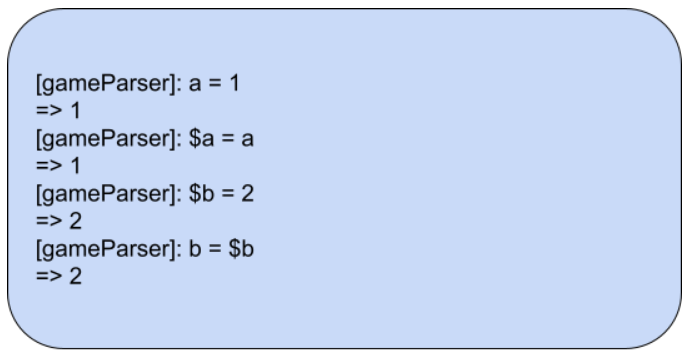
\includegraphics[scale = 0.65]{Images/Figur10.png}
  \label{}
  \caption{Deklaration av nya globala/icke-globala variabler med existerande globala/icke-globala variabler}
\end{figure}

\newpage
\subsection{Operatorer}
Gameparser inkluderar alla standardoperationer inom aritmetik, logik och jämförelser. Dessa följer de etablerade matematiska prioriteringsreglerna och logik tolkas i vänsterled. Utöver detta kan parenteser användas för ytterligare precision. Figur 11 visar några exempel på enklare aritmetiska och logiska uttryck. Se figur 12 för mer avancerade exempel som är tillåtna i Gameparser.
\begin{figure}[h!]
  \centering
  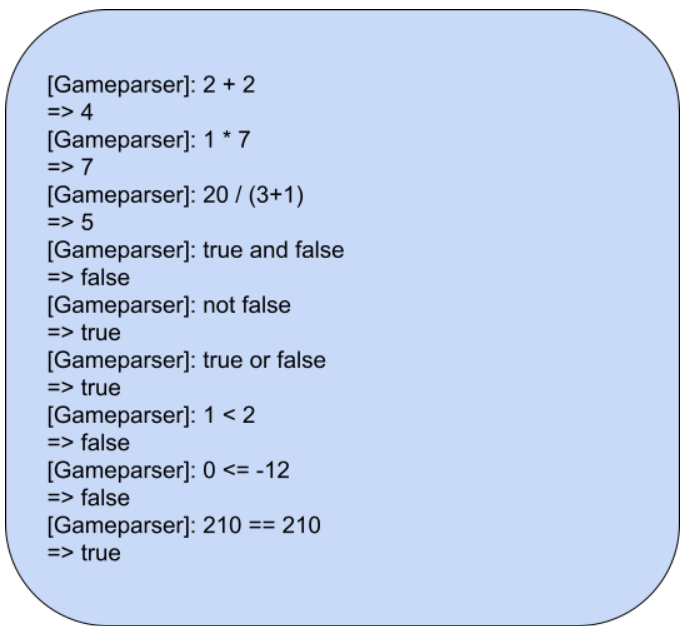
\includegraphics[scale = 0.65]{Images/Figur11.png}
  \label{}
  \caption{Exempel på enklare aritmetiska och logiska uttryck i Gameparser}
\end{figure}

\begin{figure}[h!]
  \centering
  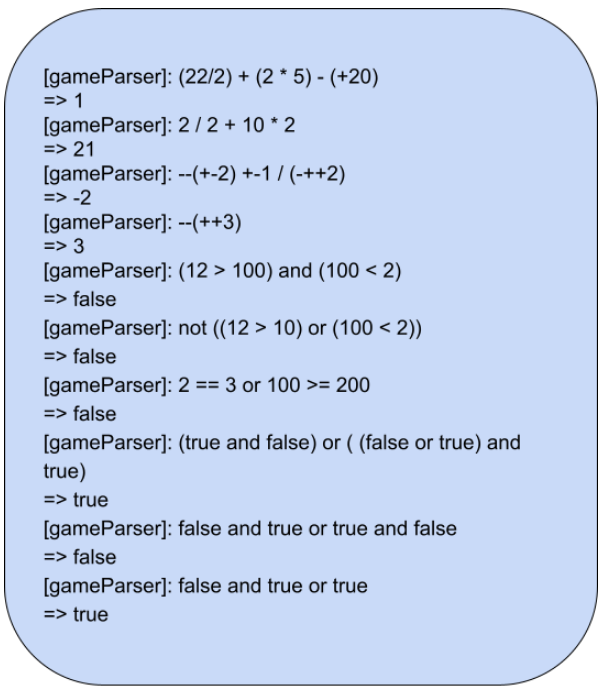
\includegraphics[scale = 0.65]{Images/Figur12.png}
  \label{}
  \caption{Mer avancerade aritmetiska och logiska uttryck}
\end{figure}

\newpage
\subsubsection{Sträng-operatorer}
I språket finns ett antal operationer som kan utföras över strängar.
Utöver vanliga operatorer som finns är det också möjligt att addera strängar. För att ha ett citattecken i en sträng ska ett \textbf{``\textbackslash''} förekomma framför citattecknet. Det gäller samma regler för \textbf{``\textbackslash n''} som representerar ny rad och \textbf{``\textbackslash t''} som representerar ett tab. \textbf{str()} kan användas för att konvertera andra datatyper till sträng. Figur 13 visar hur dessa operationer kan användas i Gameparser.

\begin{figure}[h!]
  \centering
  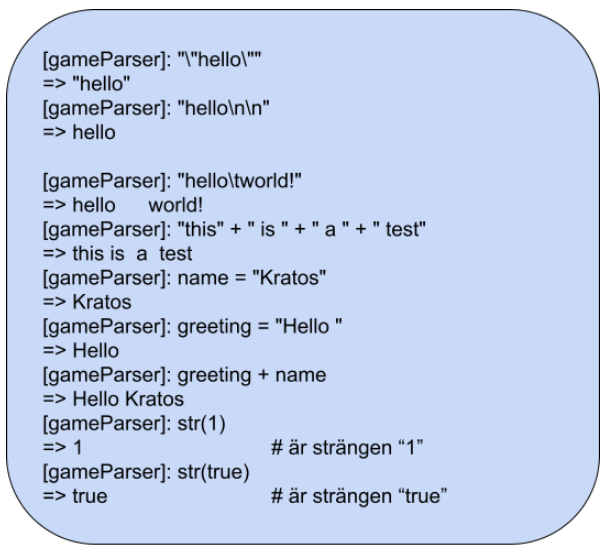
\includegraphics[scale = 0.65]{Images/Figur13.png}
  \label{}
  \caption{Exempel på sträng-operatorer}
\end{figure}


\subsubsection{List-operationer}
Gameparser har stöd för specifika operationer för att göra arbetet med listor smidigare. De grundläggande operationer som är tillgängliga är att läsa ett element i listan och skriva över ett element. Språket är noll-indexerat vilket innebär det första elementet i listan har index noll (se figur 14).

\begin{figure}[h!]
  \centering
  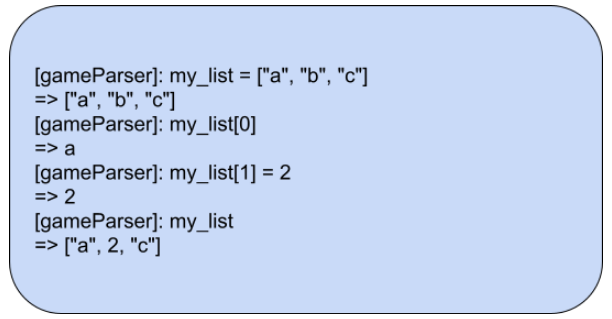
\includegraphics[scale = 0.65]{Images/Figur14.png}
  \label{}
  \caption{Tillgång till elementen i en lista}
\end{figure}

\newpage
Utöver dessa finns även följande operationer i språket:
\begin{itemize}  
\item \textbf{append:} Lägger till en element i slutet av listan ( kan båda skrivas som \textbf{my\_list.append(20)} och \textbf{my\_list <{}< 20})

\item \textbf{remove:} Tar bort ett element med det angivna indexet. Om index inte är angivet tas bort sista elementet i listan
\item \textbf{insert:} Lägger till ett element på det angivna indexet med formatet \textbf{my\_list.insert(element, index)}

\item \textbf{len:} Returnerar en heltal som motsvarar antal element i listan.
\end{itemize}

Figur 15 visar exempel på alla list-operatorer som Gameparser har stöd för.
\begin{figure}[h!]
  \centering
  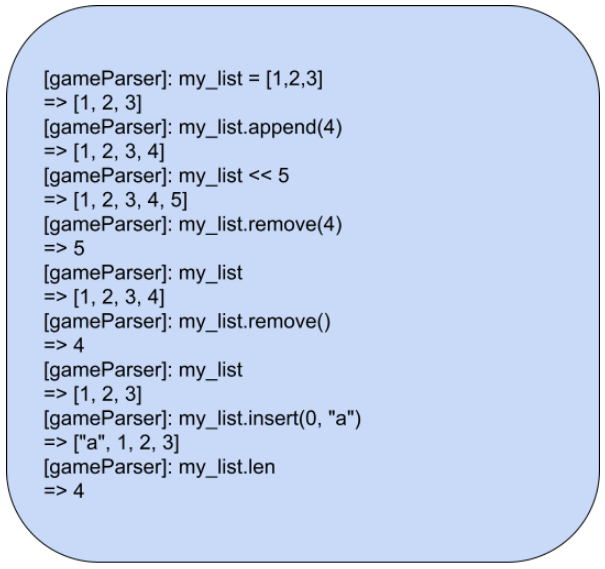
\includegraphics[scale = 0.65]{Images/Figur15.png}
  \label{}
  \caption{List-operatorer}
\end{figure}

\newpage
\subsection{In-och utmatning}
För inmatning används \textbf{read()} där en sträng kan skickas med som argument. Detta skriver eventuell sträng till terminalen och inväntar input från spelaren som sedan returneras med ENTER (se figur 16).

\begin{figure}[h!]
  \centering
  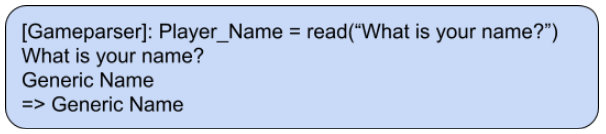
\includegraphics[scale = 0.65]{Images/Figur16.png}
  \label{}
  \caption{Inmatning}
\end{figure}

\newpage
Utmatning hanteras av \textbf{write()} som enbart skriver en sträng i terminalen. \textbf{write()} returnerar nul (se figur 17).
\begin{figure}[h!]
  \centering
  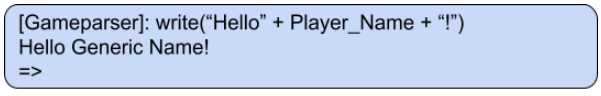
\includegraphics[scale = 0.65]{Images/Figur17.png}
  \label{}
  \caption{Utmatning}
\end{figure}

För att kunna skriva ut ett meddelande och en integer behövs en typ-konvertering från integer till sträng. Detta görs med hjälp av \textbf{str()}. Figur 18 visar hur en typ-konvertering utförs i Gameparser.
\begin{figure}[h!]
  \centering
  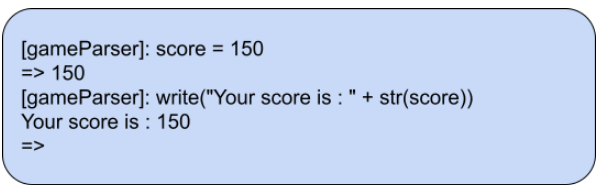
\includegraphics[scale = 0.65]{Images/Figur18.png}
  \label{}
  \caption{Typ-konvertering från heltal till sträng}
\end{figure}

\subsection{Villkor}
Villkor kan definieras med \textbf{if} eller \textbf{if} else. \textbf{if} kräver ett villkor följt av ett block som exekveras om villkoret uppfylls. \textbf{else} är en frivillig bisats som kan vara bra som alternativ då villkoret ej uppfylls. Även här krävs ett block som körs då \textbf{else} uppfylls (se figur 19).

\begin{figure}[h!]
  \centering
  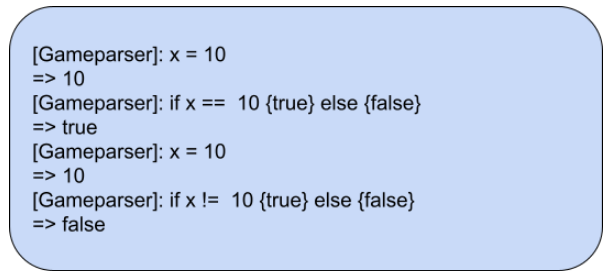
\includegraphics[scale = 0.65]{Images/Figur19.png}
  \label{}
  \caption{Exempel på hur en if-sats kan skrivas}
\end{figure}

\newpage
För fler alternativ kan \textbf{switch} användas där en variabel jämförs med flera cases för att avgöra vilket block som exekveras (se figur 20).

\begin{figure}[h!]
  \centering
  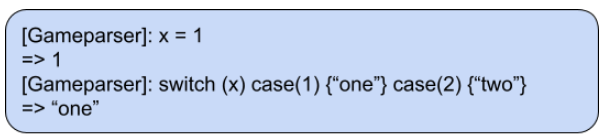
\includegraphics[scale = 0.65]{Images/Figur20.png}
  \label{}
  \caption{Exempel på hur en switch-sats kan skrivas}
\end{figure}


\subsection{Repetitionssatser}
Det finns två verktyg vilka kan använda för att implementera iteration i språket. Med en \textbf{while}-loop är det möjligt att skapa en repetitionssats som repeteras så länge ett villkor uppfylls. En \textbf{for}-loop itererar över en lista eller en range. Figur 21 visar ett exempel på en while-loop och figur 22 visar ett exempel på en for-loop.

\begin{figure}[h!]
  \centering
  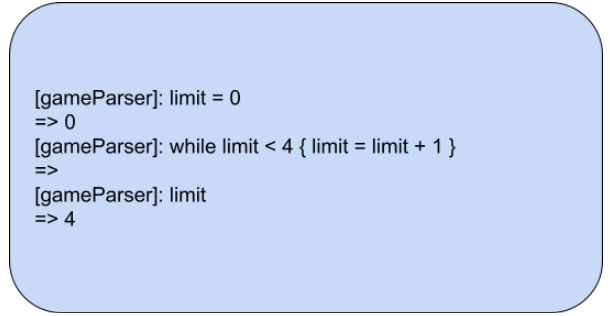
\includegraphics[scale = 0.65]{Images/Figur21.png}
  \label{}
  \caption{Exempel på while-loop}
\end{figure}

\begin{figure}[h!]
  \centering
  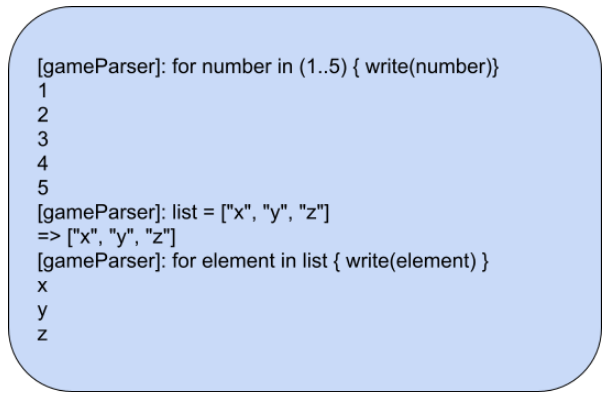
\includegraphics[scale = 0.65]{Images/Figur22.png}
  \label{}
  \caption{Exempel på for-loop}
\end{figure}

\newpage
\subsubsection{Break}
Med nyckelordet \textbf{break} kan en loop avbrytas oavsett om villkorssatsen är uppfylld eller inte (se figur 23). Oftast är det lämpligt att ha en if-sats för att se om ett mål har uppnåtts och om det är så används \textbf{break} för att avsluta iterationen. \textbf{break} kan vara mycket användbar när det gäller oändliga loopar.

\begin{figure}[h!]
  \centering
  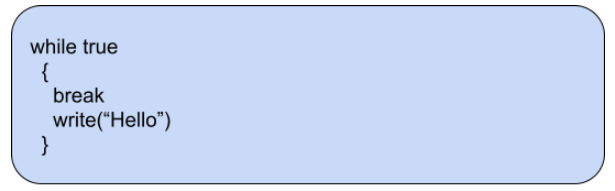
\includegraphics[scale = 0.65]{Images/Figur23.png}
  \label{}
  \caption{While-loopen avslutas utan någon utskrif}
\end{figure}

\newpage
I figur 24 visas ett praktiskt exempel på hur en \textbf{break} kan vara användbar när det gäller en oändlig while-loop. Figur 25 visar att det går lika bra att använda \textbf{break} i en range-baserade for-loop.

\begin{figure}[h!]
  \centering
  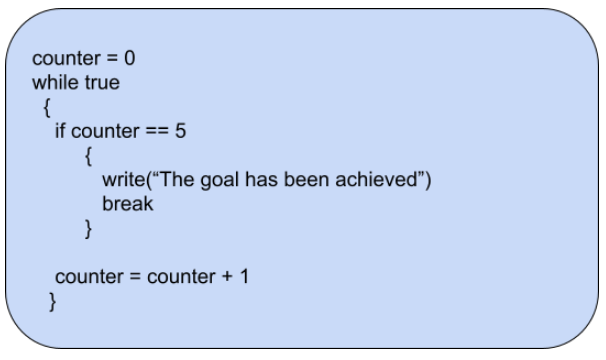
\includegraphics[scale = 0.65]{Images/Figur24.png}
  \label{}
  \caption{Break inuti if-satsen avslutar while-loopen}
\end{figure}

\begin{figure}[h!]
  \centering
  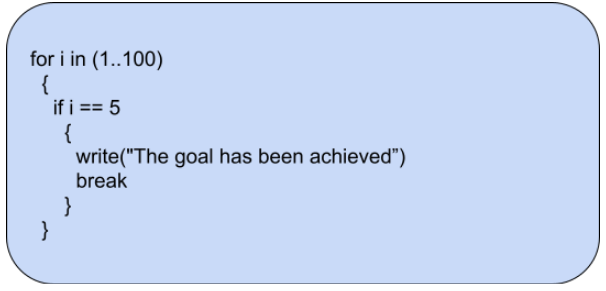
\includegraphics[scale = 0.65]{Images/Figur25.png}
  \label{}
  \caption{Break inuti if-satsen avslutar for-loopen}
\end{figure}

\newpage
\subsection{Funktioner}
Gameparser har stöd för användardefinierade funktioner. I figur 26 ser ni ett exempel på en enkel funktion som beräknar summan av två parameter och returnerar resultatet.
\begin{figure}[h!]
  \centering
  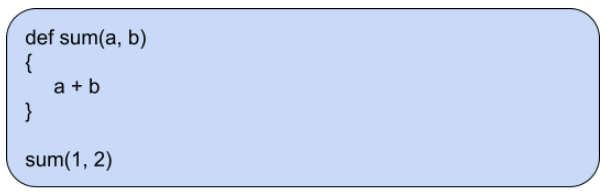
\includegraphics[scale = 0.65]{Images/Figur26.png}
  \label{}
  \caption{En funktion som returnerar summan av två parameter ( returnerar 3 i det här fallet)}
\end{figure}

Funktioner som definieras i programmet är tillgängliga globalt och är inte beroende på scope.
Språket däremot inte tillåter att en funktion definieras inuti en annan funktion (nästling). Figur 27 visar ett otillåtet fall som ska undvikas när det gäller definition av funktioner. 

\begin{figure}[h!]
  \centering
  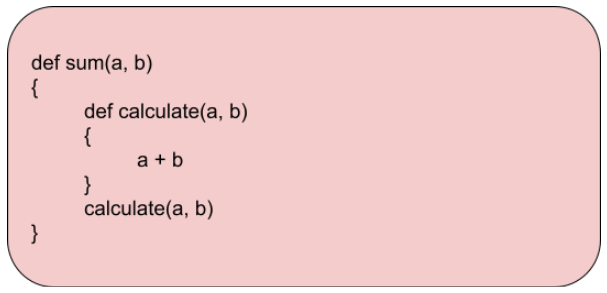
\includegraphics[scale = 0.65]{Images/Figur27.png}
  \label{}
  \caption{En funktion får \textbf{inte} definieras i en annan funktion i Gameparser}
\end{figure}

\newpage
\subsubsection{Rekursion}
Stöd för rekursion låter programmeraren anropa en funktion inuti definitionen om och om igen. Med hjälp av rekursion löses vissa problem mycket effektivare jämfört med andra metoder och därför har detta implementerats i Gameparser. Figur 28 visar implementationen av funktionen ``Fib'' som räknar motsvarande Fibonacci-tal.

\begin{figure}[h!]
  \centering
  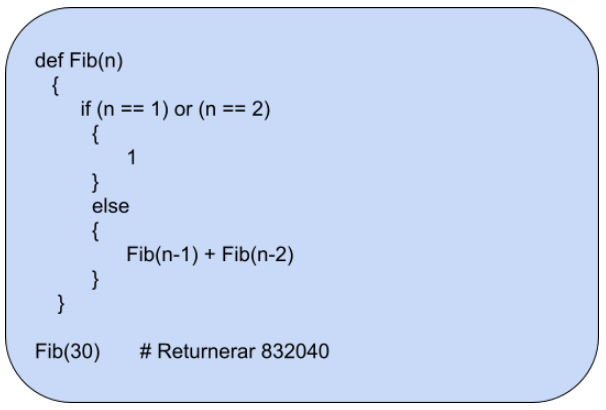
\includegraphics[scale = 0.65]{Images/Figur28.png}
  \label{}
  \caption{Funktionen som beräknar Fibonacci-talet för ett angivet tal}
\end{figure}


\subsection{Enkla klasser}
Gameparser erbjuder två konstruktioner som skiljer det från andra liknande språk. Dessa verktyg är avsedda för att göra det enklare för programmeraren att skapa ett textbaserat spel utan att t.ex. behöva skriva så många nästlade if-satser.

\subsubsection{event}
Den här konstruktorn motsvarar ett vägskäl där spelaren ges alternativ med vilket sedan programmet körs vidare. Ett event kan exempelvis representeras som ett skog där spelaren får veta om situationen där och får välja vad denne ska göra. Ett event består av två huvuddelar: \textbf{init} och \textbf{run}. Init är till för att initiera event. Där kan lokala variabler initieras med ett önskad startvärde. All kod inuti init körs \textbf{en gång} när spelet för första gången anropar eventet. Run-delen är tänkt att vara kroppen av eventet där programmeraren kan bestämma vad som ska hända. Till exempel är det möjligt att skriva ut lite text för att informera spelaren om situationen. Sedan kan inmatningen läsas med hjälp av read och en villkorssats kan bestämma hur programmet ska ta sin väg till en lämplig konsekvens.
Det är ganska fritt i init/run-delen när det gäller kod. Programmeraren har i stort sett tillgång till nästan alla konstruktioner såsom repetitionssatser, villkorssatser, funktionsanrop, tillgång till globala variabler o.s.v. Distinktionen är att init initierar eventet. Däremot är det inte tillåtet att definiera en funktion eller en annan klass inuti ett event. Figur 29 visar ett enkelt exempel på hur en eventklass kan konstrueras.

\begin{figure}[h!]
  \centering
  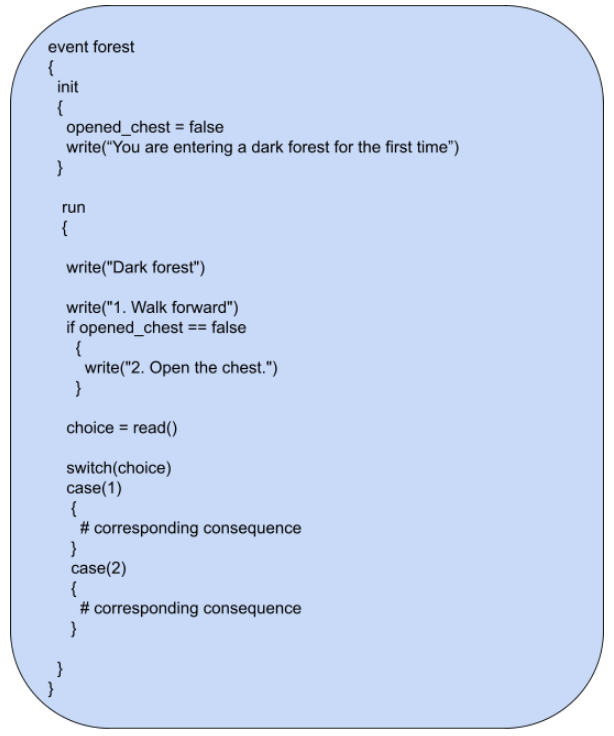
\includegraphics[scale = 0.65]{Images/Figur29.png}
  \label{}
  \caption{Implementering av ett event}
\end{figure}

\newpage
Efter att ett event har skapats går det att ladda eventet med hjälp av den reserverade funktionen \textbf{load()}.
Observera att ett event inte beroende på scope och kan kallas var som helst i koden.  \textbf{load()} tar ett event som argument och eventuellt filnamnet på en bild (jpg eller png) placerad i images-mappen  (se figur 30). Denna bild visas då  \textbf{load()} körs. Bilden stängs med Escape.

\begin{figure}[h!]
  \centering
  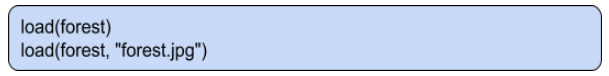
\includegraphics[scale = 0.65]{Images/Figur30.png}
  \label{}
  \caption{load() används för att köra ett event}
\end{figure}

Resultatet av första körningen visas i figur 31.

\begin{figure}[h!]
  \centering
  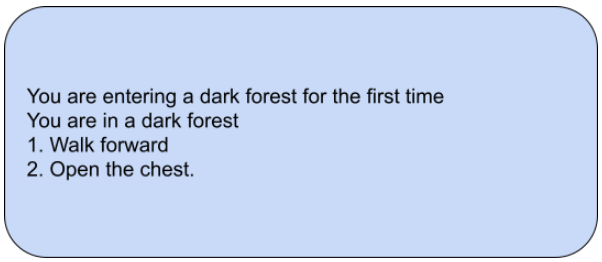
\includegraphics[scale = 0.65]{Images/Figur31.png}
  \label{}
  \caption{Visar hur event ``forest'' ser ut när den körs för första gången}
\end{figure}

\newpage
Notera att om eventet laddas för andra gången skrivs inte första raden ut som finns i init-delen (se figur 32).

\begin{figure}[h!]
  \centering
  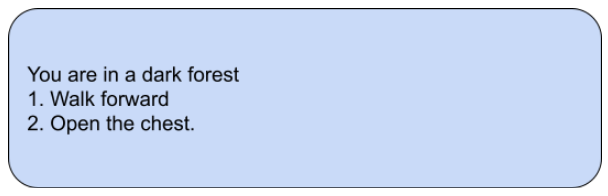
\includegraphics[scale = 0.65]{Images/Figur32.png}
  \label{}
  \caption{Visar hur event ``forest'' ser ut när den körs för andra gången}
\end{figure}

\newpage
\subsubsection{prop}
Denna konstruktor används för att skapa abstrakta objekt som kan innehålla en eller flera datamedlemmar. Det finns ingen run-del, istället det går att definiera en parameterlista för att sedan kunna skapa en instans av klassen med godtyckliga värden.


En instansiering av en prop görs genom att använda nyckelordet \textbf{``new''}. Efter att en instans har skapats går det att komma åt dess datamedlemmar med en punkt. Figur 33 visar ett exempel på definition samt instansiering av ett \textbf{prop}.

\begin{figure}[h!]
  \centering
  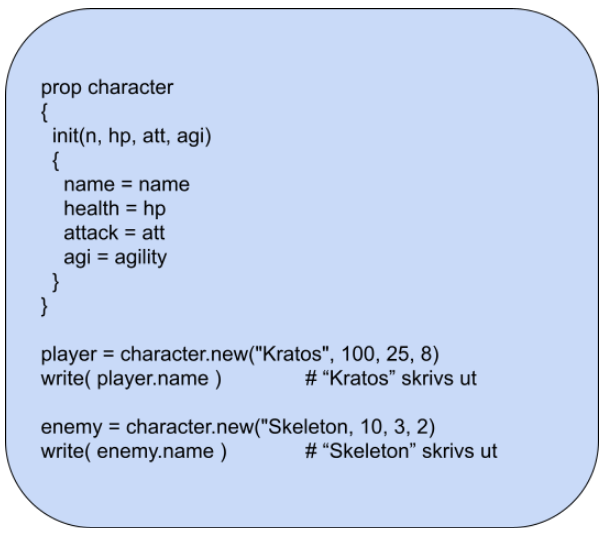
\includegraphics[scale = 0.65]{Images/Figur33.png}
  \label{}
  \caption{Exempel på hur ett prop kan definieras och instansieras}
\end{figure}

Notera att oftast behöver ett spelar-objekt nås i olika event och funktioner i spelet. Därför är det lämpligt att spelar-objektet deklareras globalt (se figur 34).

\begin{figure}[h!]
  \centering
  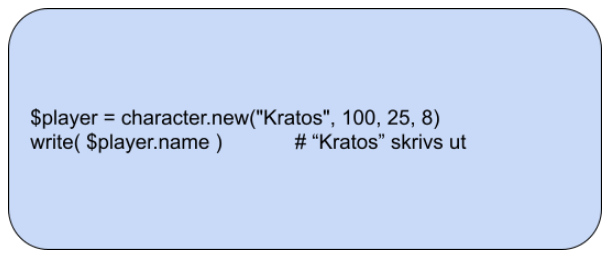
\includegraphics[scale = 0.65]{Images/Figur34.png}
  \label{}
  \caption{Spelar-objektet skapas med fördel som globalt}
\end{figure}

\newpage
\subsection{Scope}
Scope hanteras internt via hashtabeller i en lista Varje scope har ett heltal som korrelerar med en av hashtabellerna där dess variabler lagras. En variabel i t.ex. en funktion kan därför inte nås från ett annat scope (se exemplet i figur 35). För detta krävs globala variabler.

\begin{figure}[h!]
  \centering
  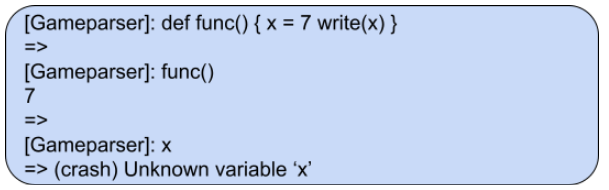
\includegraphics[scale = 0.65]{Images/Figur35.png}
  \label{}
  \caption{Funktioner har egna lokala variabler som inte är tillgängliga utanför funktions-blocket}
\end{figure}

Samtliga funktionsvariabler är definierade inom funktions-ramen mellan måsvingar och programmeraren har friheten att använda och ändra variabeln utan att den påverkar andra variabler med samma namn i ett annat scope. Figur 36 visar ytterligare exempel på detta.

\begin{figure}[h!]
  \centering
  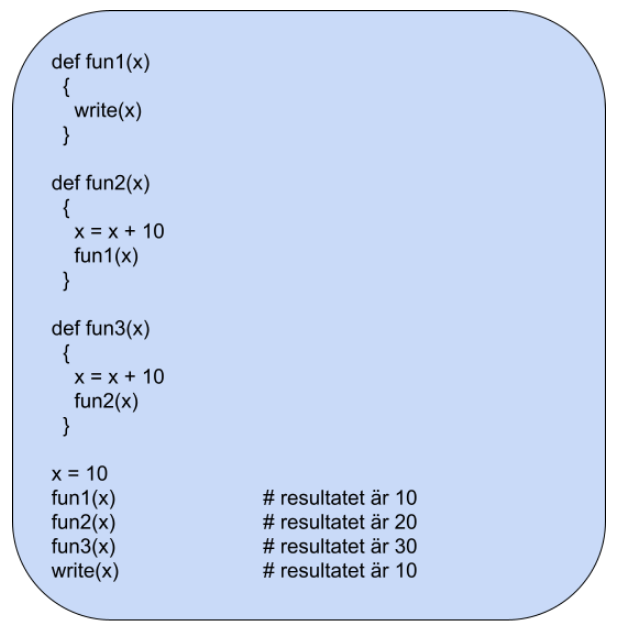
\includegraphics[scale = 0.65]{Images/Figur36.png}
  \label{}
  \caption{Scope-hantering i Gameparser}
\end{figure}

\newpage
Det gäller samma princip för definitionen av ett event och prop och deras variabler och data medlemmar kan inte kommas åt från ett annat scope.

\subsection{Andra fördefinierade funktioner}
Förutom de fördefinierade funktioner som förklarades ovan (\textbf{write()}, \textbf{read()}, \textbf{load()} och \textbf{str()}) finns det två ytterligare funktioner som kan vara användbara när det gäller textbaserad spelprogrammering:

\begin{itemize}  
\item \textbf{wait():} som är för att pausa körningen av spelet för ett antal sekunder
\item \textbf{cls():} som rensar terminalen.
\end{itemize}

\newpage
\section{Systemdokumentation}
\subsection{Lexer}
Den lexikaliska analysen bygger på att rdparse delar upp inläst kod i “tokens” utifrån reguljära uttryck. Först rensas koden på kommentarer och blanktecken. Sedan identifieras reserverade ord samt alla tillgängliga datatyper. Dessa tokens lämnas till sist över till parsern.

\subsection{Parser}
Gameparser använder rdparse för sekventiellt bearbeta inlästa tokens. De sammankopplas till ett abstrakt syntaxträd.

\subsection{Abstrakt syntaxträd}
Nu består programmet av långa grenar rotade ur programmet som helhet. Varje spets har specificerats till en datatyp. Varje förgrening kan ses som en nod där ett objekt skapas med en init- och en eval-funktion. De två verktygen låter parsern först bygga upp trädet och sedan exekvera koden strukturerat. Retursatser klättrar längs med grenarna tills slutligen den sista kodraden bearbetats.

\subsection{Kodstandard}
Det finns ingen specificerad kodstandard utöver de krav som tidigare nämnts. Block skapas inom måsvingar, variabelnamn inleds med bokstäver och globala variabler inleds med \textbf{\$}-tecken.

\subsection{BNF}

\begin{tabbing}
  \= {} {} {} {} {} {} {} {} {} {} {} {} {} {} {} {} {} {} {} {} {} {} {} {} {} {} {} \= {} {} {} {} {} {} {} {} {} {} {} {} {} {} {} {} {} {}\= \\
  \><prog> \>::= \><comps> \\\\
  \><comps>  \>::= \><comps> <comp>\\
  \> \> | \> <comp> \\\\

  \><comp> \>::= \><definition>\\
  \> \>| \><statement>\\\\

  \><definition> \>::= \><prop>\\
  \> \>| \> <event> \\
  \> \>| \> <function\_def>\\\\

  \><prop> \>::= \>\textbf{prop} \textcolor{Cyan}{Identifier} { <init> }\\\\

  \><event> \>::= \>\textbf{event} \textcolor{Cyan}{Identifier} { <init> \textbf{run} <block> }\\\\

  \><init> \>::= \>\textbf{init} \textbf{(} <params> \textbf{)} <block>\\
  \> \>| \> \textbf{init} <block>\\\\

  \><function\_def>\>::= \>\textbf{def} \textcolor{Cyan}{Identifier} \textbf{(} <params> \textbf{)} <block>\\\\

  \><params> \>::= \><params> \textbf{,} <param>\\
  \> \>| \> <param>\\
  \> \>| \> <empty>\\\\

  \><param> \>::= \><identifier>\\\\

  \><block> \>::= \>{ <statements> }\\
  \> \>| \> { <empty> }\\\\

  \><function\_call> \>::= \>\textcolor{Cyan}{Identifier} \textbf{(} <values> \textbf{)}\\
  \> \>| \> \textbf{write (} \textcolor{Cyan}{Identifier} \textbf{)}\\
  \> \>| \> \textbf{write (} \textcolor{Cyan}{GIdentifier} \textbf{)}\\
  \> \>| \> \textbf{write (} <exp> \textbf{)}\\
  \> \>| \> \textbf{write ( )}\\
  \> \>| \> \textbf{read} \textbf{(} <exp> \textbf{)}\\
  \> \>| \> \textbf{read ( )}\\
  \> \>| \> \textbf{wait (} \textcolor{orange}{Integer} \textbf{)}\\
  \> \>| \> \textbf{load (} \textcolor{Cyan}{Identifier}\textbf{,} <exp> \textbf{)}\\
  \> \>| \> \textbf{load (} \textcolor{Cyan}{Identifier} \textbf{)}\\
  \> \>| \> \textbf{str (} <exp> \textbf{)}\\
  \> \>| \> \textbf{cls ( )}\\\\


  \><statements> \>::= \><statements> <statement>\\
  \> \>| \> <statement>\\\\

  \><statement> \>::= \><condition>\\
  \> \>| \> <loop>\\
  \> \>| \> <assignment>\\
  \> \>| \> <array\_op>\\
  \> \>| \> <exp>\\
  \> \>| \> \textcolor{blue}{Break}\\\\

  \><assignments> \>::= \><assignments> <assignment>\\
  \> \>| \> <assignment>\\\\

  \><assignment> \>::= \><identifier> \textbf{=} <array\_op>\\
  \> \>| \> <identifier> \textbf{=} <exp>\\
  \> \>| \> <identifier> \textbf{[} \textcolor{orange}{Integer} \textbf{]} \textbf{=} <exp>\\
  \> \>| \> <identifier> \textbf{.} \textcolor{Cyan}{Identifier}  \textbf{=} <exp>\\\\

  \><exp> \>::= \><bool\_exp> \textbf{and} <exp>\\
  \> \>| \> <bool\_exp> \textbf{or} <exp>\\
  \> \>| \> \textbf{not} <exp>\\
  \> \>| \> <bool\_exp>\\\\

  \><bool\_exp> \>::= \><math\_exp> CompOp <math\_exp>\\
  \> \>| \> <bool\_val> CompOp <bool\_val>\\
  \> \>| \> <bool\_val>\\\\

  \><bool\_val> \>::= \>\textbf{\textcolor{ForestGreen}{true}}\\
  \> \>| \> \textbf{\textcolor{red}{false}}\\
  \> \>| \> <math\_exp>\\\\

  \><math\_exp> \>::= \><math\_exp> \textbf{+} <term>\\
  \> \>| \> <math\_exp> \textbf{-} <term>\\
  \> \>| \> <term>\\\\

  \><term> \>::= \><term> \textbf{*} <factor>\\
  \> \>| \> <term> \textbf{/} <factor>\\
  \> \>| \> <factor>\\\\

  \><factor> \>::= \>\textcolor{orange}{Integer} \\
  \> \>| \> <signs> \textcolor{orange}{Integer}\\
  \> \>| \> <signs> \textbf{(} <math\_exp> \textbf{)}\\
  \> \>| \> \textbf{(} <exp> \textbf{)}\\
  \> \>| \> <function\_call>\\
  \> \>| \> <array>\\
  \> \>| \> <instancing>\\
  \> \>| \> <instance\_reader>\\
  \> \>| \> <variable\_node>\\
  \> \>| \> \textcolor{ForestGreen}{LiteralString}\\
  \> \>| \> \textcolor{Purple}{Range}\\\\

  \><signs> \>::= \><signs> <sign>\\
  \> \>| \> <sign>\\\\

  \><sign> \>::= \>\textbf{+}\\
  \> \>| \> \textbf{-}\\\\

  \><array> \>::= \><identifier> \textbf{[} \textcolor{orange}{Integer} \textbf{]}\\
  \> \>| \> \textbf{[} <values> \textbf{]}\\
  \> \>| \> \textbf{[} \textbf{]}\\\\

  \><array\_op> \>::= \><identifier> <operations>\\
  \> \>| \> <array> <operations>\\
  \> \>| \> <instance\_reader> <operations>\\
  \> \>| \> <:function\_call> <operations>\\\\

  \><operations> \>::= \><operations> <operation>\\
  \> \>| \> <operation>\\\\

  \><operation> \>::= \>\textbf{[} \textcolor{orange}{Integer} \textbf{]}\\
  \> \>| \> \textbf{. remove (} <exp> \textbf{)}\\
  \> \>| \> \textbf{. remove ( )}\\
  \> \>| \> \textbf{. append (} <exp> \textbf{)}\\
  \> \>| \> \textbf{. append <{}<} <exp>\\
  \> \>| \>  \textbf{. insert (} \textcolor{orange}{Integer} \textbf{,} <exp> \textbf{)}\\
  \> \>| \>  \textbf{. len}\\\\

  \><values> \>::= \><values> \textbf{,} <exp>\\
  \> \>| \> <exp>\\
  \> \>| \> <empty>\\\\

  \><instancing> \>::= \><identifier> \textbf{. new} \textbf{(} <values> \textbf{)}\\\\

  \><instance\_reader> \>::= \><identifier> \textbf{.} <identifier>\\\\

  \><condition> \>::= \><if>\\
  \> \>| \>  <switch>\\\\

  \><if> \>::= \>\textbf{if}  <exp> <block> \textbf{else} <block>\\
  \> \>| \> \textbf{if} <exp> <block>\\\\

  \><switch> \>::= \>\textbf{switch} \textbf{(} <exp> \textbf{)} <cases>\\\\

  \><cases> \>::= \><cases> <case>\\
  \> \>| \> <case>\\\\

  \><case> \>::= \>\textbf{case} \textbf{(} <exp> \textbf{)} <block>\\\\

  \><loop> \>::= \>\textbf{while} <exp> <block>\\
  \> \>| \> \textbf{for} \textcolor{Cyan}{Identifier} \textbf{in} \textcolor{Purple}{Range} <block>\\
  \> \>| \> \textbf{for} \textcolor{Cyan}{Identifier} \textbf{in} <array> <block>\\
  \> \>| \> \textbf{for} \textcolor{Cyan}{Identifier} \textbf{in} \textcolor{Cyan}{Identifier} <block>\\
  \> \>| \> \textbf{for} \textcolor{Cyan}{Identifier} \textbf{in} \textcolor{Cyan}{GIdentifier} <block>\\\\

  \><identifier> \>::= \>\textcolor{Cyan}{Identifier} \\
  \> \>| \> \textcolor{Cyan}{GIdentifier}\\\\

  \><variable\_node> \>::= \>\textcolor{Cyan}{Identifier} \\
  \> \>| \> \textcolor{Cyan}{GIdentifier}\\
\end{tabbing}
\newpage
\section{Reflektion}
Projektet lyckades utan större svårigheter hålla sig inom de uppsatta tidsramarna. Den del som främst utmärkte sig var då scope och funktioner skulle implementeras. Dessa element visade sig vara sammanbundna och därmed till stor del ömsesidigt beroende.\\

Orginalplanen var inte att implementera funktioner men allt eftersom projektet fortgick blev behovet av dessa uppenbart. Detta krävde en del arbete men när det väl var genomfört gick implementationen av rekursion smidigt. Det som var svårt med funktionsimplementationen var att det kändes förvirrande att skapa klasser och noder för senare användning. Körningen av kod i run-time ledde till att programmet inte kördes pålitligt och eftersom testningen i början främst fokuserat på interaktivt läge märktes det inte att kod med flera rader inte lyckades köras. Lösningen var att bryta ut kod som ska köras till evaluate-delen i motsvarande klass.\\

När dessa hinder övervunnits fann projektet sig plötsligt framför utlagt tidsplan vilket lämnade rum för mer finputsning i slutskedet.


\end{document}
